\chapter{Dinamica del veicolo}
\label{cha:cap1}
 
Questo capitolo vuole essere un introduzione alla dinamica del veicolo,
che è la disciplina che studia e applica i principi della dinamica allo studio del moto dei veicoli terrestri, per analizzarne l'interazione con le cause che determinano e modificano il comportamento dello stesso.\\
Illustreremo e evidenzieremo i fondamenti di dinamica laterale che governano il comportamento in curva di semplici modelli di veicoli in condizioni stazionarie,  
con enfasi sull'influenza delle caratteristiche del pneumatico.\\
Verranno analizzati gli effetti sulla risposta del veicolo, di vari fattori che caratterizzano gli pneumatici.

\section{Pneumatici}
Lo pneumatico è uno dei componenti più 
importanti dell’autoveicolo e di tutti i veicoli
stradali in genere.
Nonostante siano in continua evoluzione il loro ruolo e la loro importanza rimarranno sempre fondamentali all'interno di un veicolo.\\
Essi rappresentano gli unici punti di contatto del veicolo con il suolo, e sono responsabili della generazione delle 
forze laterali necessarie alla tenuta in curva, e delle forze longitudinali necessarie alla trazione  e alla frenata del veicolo.\\
La deformabilità del pneumatico rappresenta la sua caratteristica più importante, essa rende possibile il mantenimento del contatto ruota-strada nonostante le rugosità e asperità del piano di contatto.\\
La deformabilità laterale e longitudinale garantisce la generazione di forze mentre la deformabilità radiale contribuisce a migliorare il comfort di marcia.\\
Di particolare importanza risulterà
la pendenza della curva di forza laterale Fy rispetto all'angolo di deriva, chiamata Cornering stiffness: è un parametro fondamentale per quanto riguarda la risposta del pneumatico e sta alla base delle analisi di risposta dei veicoli.
Le eventuali non linearità della caratteristica dei pneumatici definiscono  
le proprietà di manovrabilità e stabilità del veicolo ad accelerazioni laterali più elevate.
Il trasferimento di carico in curva unito alla dipendenza della caratteristica del pneumatico rispetto al carico radiale
agente sullo stesso, ha un effetto considerevole sul caratteristiche di manovrabilità dell'auto.

\subsection{Introduzione ai pneumatici}
Gli pneumatici sono il solo legame tra il veicolo e strada. Le prestazioni di un autoveicolo sono largamente influenzate dalle caratteristiche di aderenza e deformabilità dei pneumatici utilizzati.
Per capirne l’importanza, occorre considerare che il controllo dell’equilibrio e del moto del veicolo avviene grazie alla generazione di forze longitudinali e laterali, agenti all’interno delle impronte di contatto dello pneumatico con il piano stradale. Le forze nascono come risultato dell’azione effettuata dal conducente attraverso il meccanismo di sterzo, l’acceleratore ed il sistema frenante, ma sopratutto come reazione alla forza centrifuga proporzionale all'accellerazione laterale, che spinge il veicolo verso l'esterno durante una curva.


\subsubsection{Struttura dei pneumatici }
I pneumatici sono composti da numerose parti con ruoli e materiali differenti.
Questa struttura fortemente composita dona le caratteristiche di deformabilità ed aderenza richieste.
L'aria presente all'interno dei pneumatici conferisce stabilità e rigidezza all'insieme mantenendo valori di massa contenuti.
\begin{figure}[ht]
    \centering
    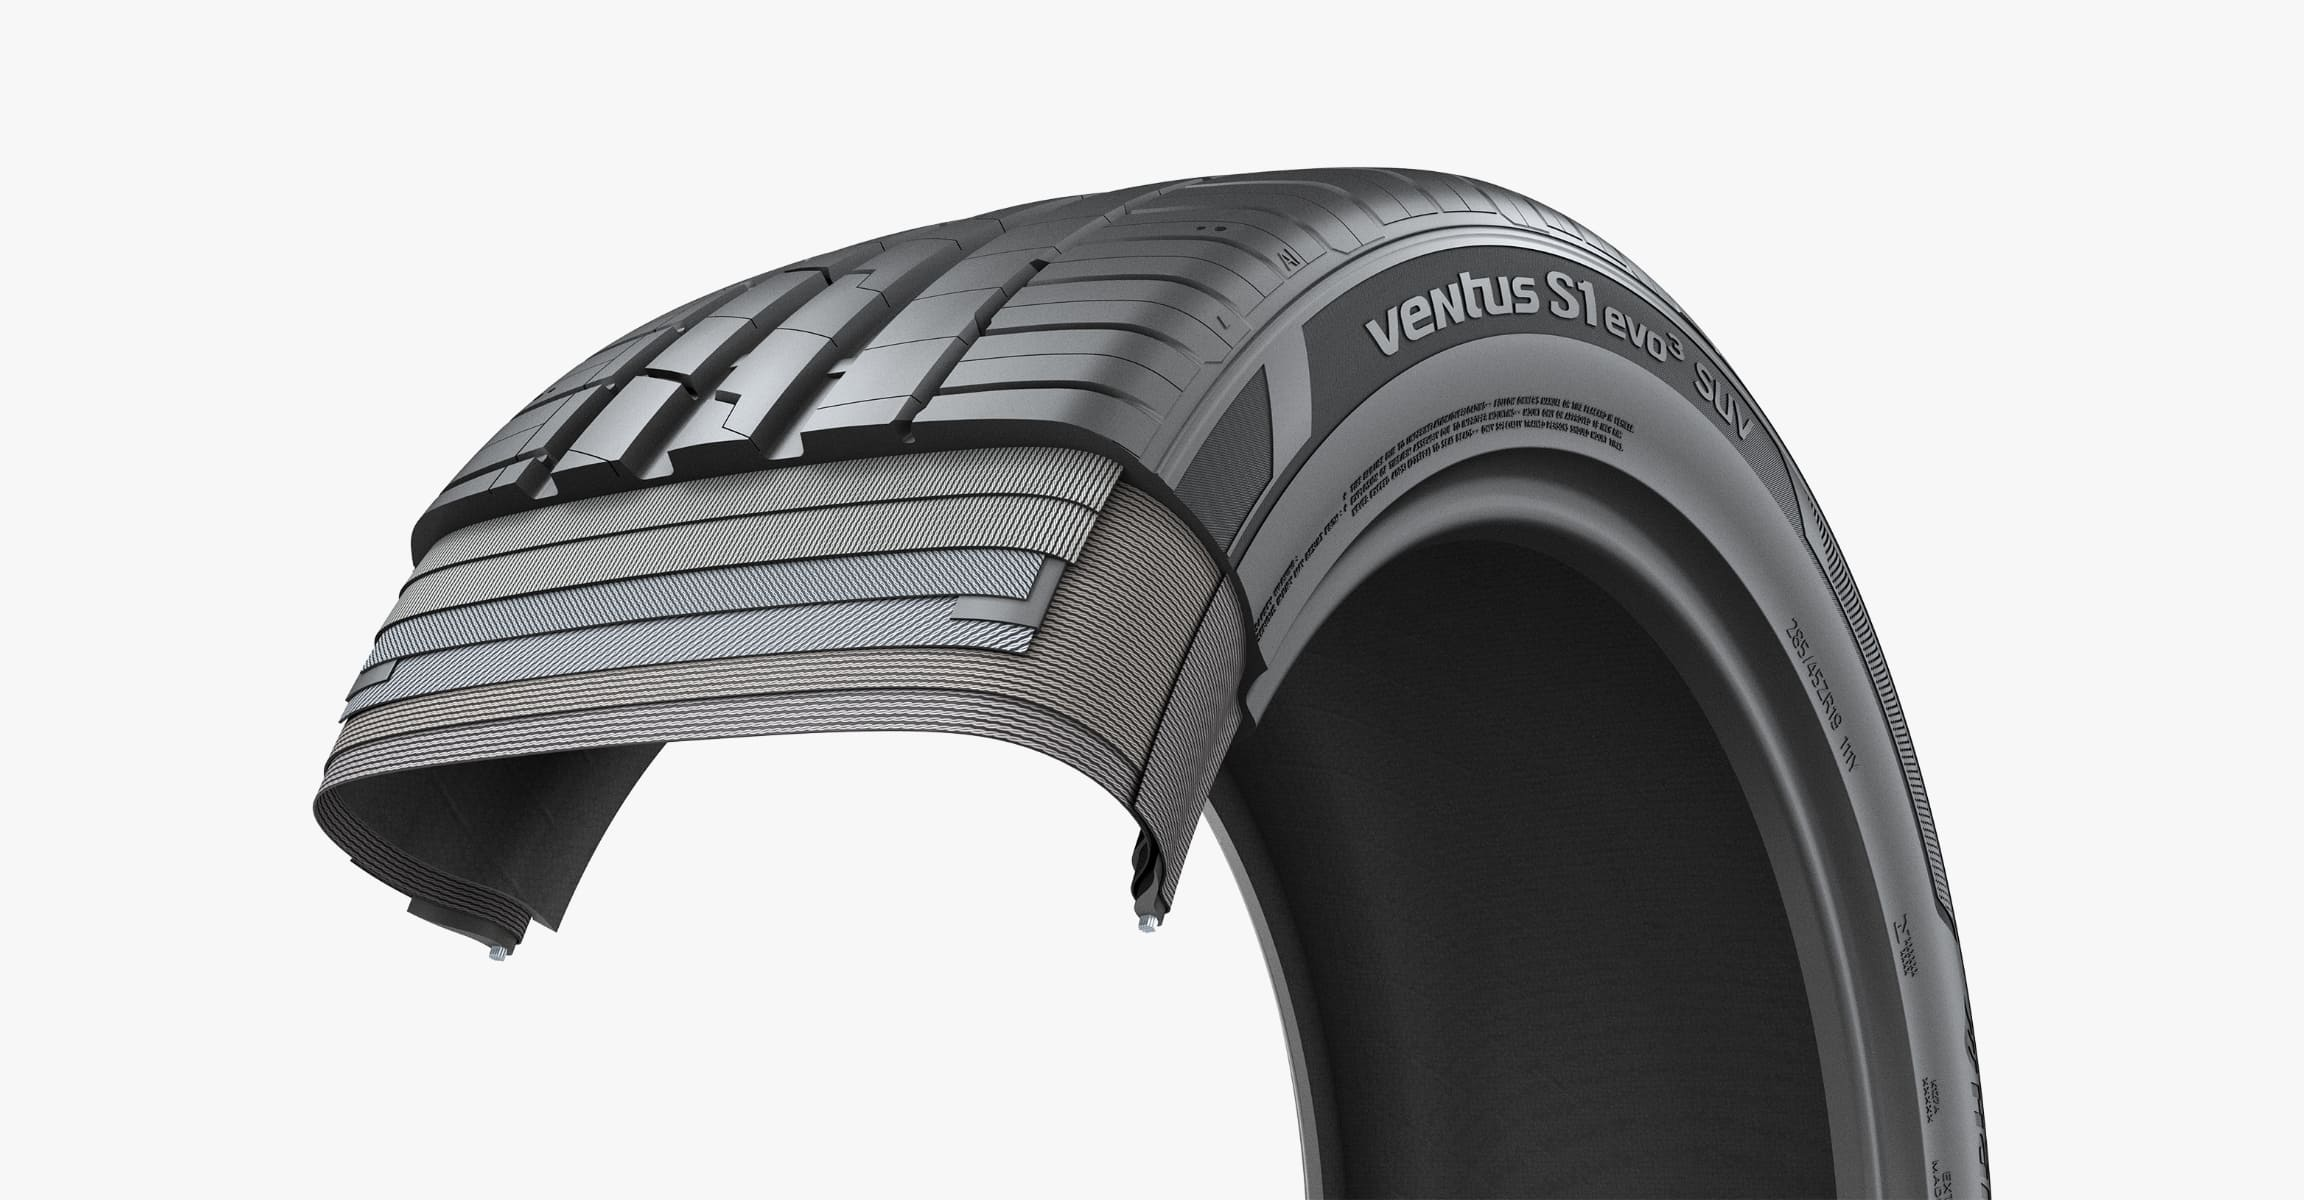
\includegraphics[scale=0.15]{Immagini/Tyres/Tire Structure_w.jpg}
    \caption{Struttura del pneumatico}
    \label{fig:Structure_tyres}
\end{figure}
\begin{description}
    \item[Carcassa :] è la parte più importante perchè rappresenta il telaio dello pneumatico. Il termine carcassa indica tutti gli strati composti dalle nappe a trama dello pneumatico. Assorbe la pressione dell'aria interna allo pneumatico, il peso e i colpi.
    \item [Strato intermedio e cintura :]
    è una struttura a nido d‘ape realizzata con fili di ferro collocata (diagonalmente) tra il battistrada e la carcassa, al fine di proteggere quest'ultima. Assorbe i colpi esterni e impedisce alle scheggiature o alle lesioni al battistrada di venire a diretto contatto con la carcassa. Allo stesso tempo, previene la separazione dello strato di gomma e della carcassa. La cintura ,invece, è un forte strato di rinforzo collocato nella circonferenza tra il battistrada e la carcassa negli pneumatici radiali e cinturati. Le funzioni della cintura sono simili a quelle dello strato intermedio; inoltre, rinforza la solidità del battistrada serrando saldamente la carcassa.
    \item [Spalla :] è la parte di pneumatico collocata tra il battistrada e la parete laterale, essa è composta dallo strato di gomma più spesso dell'intero pneumatico. Ha il compito di garantire la stabilità in curva e mantenere la traiettoria durante la guida.
    \item [Battistrada :] è composto da uno spesso strato di gomma che viene direttamente a contatto con la superficie stradale. È altamente resistente alla rottura e ai colpi, al fine di proteggere la carcassa e la cintura all'interno dello pneumatico. 
    il disegno dello stesso e la mescola di cui è composto sono caratteristica fondamentali che definiscono le prestazioni del pneumatico stesso .
    \item [Parete Laterale :] è collocata tra la spalla e il tallone, ha il compito di proteggere la carcassa e di aumenta le prestazioni di guida attraverso la sua flessibilità.
    \item [Tallone :] Ha il compito di fissare lo pneumatico al cerchione. È formato da varie parti, comprendenti il filo del tallone, il nucleo, la gomma e l'aletta. In generale, il cerchione è leggermente stretto, in modo che, in caso di riduzione improvvisa della pressione dell'aria durante la guida, lo pneumatico non si stacchi improvvisamente dal cerchione.
    \item [Liner interno :]
     consiste in uno strato di gomma con delle qualità ermetiche elevate. La gomma è generalmente composta di butile, da gomma sintetica o da un tipo di poli-isoprene. La funzione principale è quella di mantenere l'aria all'interno dello pneumatico.
\end{description}



\subsubsection{L'effetto del carico verticale}
La pressione media al suolo nell’area di contatto è, in prima approssimazione,
pari alla pressione di gonfiaggio del pneumatico

Il pneumatico, gonfiato ad una pressione p e soggetto ad un carico verticale $F_z$, si deformerà in modo tale da mettere in contatto con il suolo una superficie pari al rapporto $F_z / p$.
Questa deformazione comporterà uno schiacciamento pari ad f.
Più alto è il carico e più bassa è la pressione maggiore sarà la deformazione.

\subsubsection{Caratterizzazione dei pneumatici}
L'analisi del comportamento meccanico dei pneumatici si basa spesso sui risultati ottenuti sperimentalmente su singole gomme.\\
Per caratterizzare il pneumatico rispetto al comportamento direzionale si suppone che la superficie sia perfettamente piana e orizzontale.
Questo tipo di prove sono spesso svolte appoggiando la ruota su un tappeto mobile o su un tamburo rotante con superficie abrasiva.\\
Il sistema consiste in una macchina a disco rotante capace di misurare le forze e i momenti
agenti sullo pneumatico in seguito all’assegnazione di determinati valori di angoli di deriva,
di rollio e carico verticale.\\
Nonostante nessuna di queste prove standard corrisponde alle effettive condizioni di utilizzo i dati ottenuti sono comunque molto utili.
Essi sono di fondamentale importanza poichè nell'ultimo ventennio le simulazioni virtuali di veicoli sono diventate la base per la progettazione e l'ottimizzazione di veicoli.
Questi dati dovrebbero avere un accuratezza abbastanza elevata in modo da garantire una buona attendibilità delle simulazioni, con il passare degli anni sono stati sviluppati modelli empirici sempre più sofisticati in grado di avvicinarsi sempre maggiormente alla realtà.
Tuttavia non sempre i fornitori sono disposti a fornire dati accurati e completi per quanto riguarda i loro prodotti e spesso risultano difficili da reperire.

\subsection{Forze e slip}
Un pneumatico può essere descritto come un sistema in grado di generare forze e momenti come conseguenza degli input applicati.
\begin{figure}[ht]
    \centering
    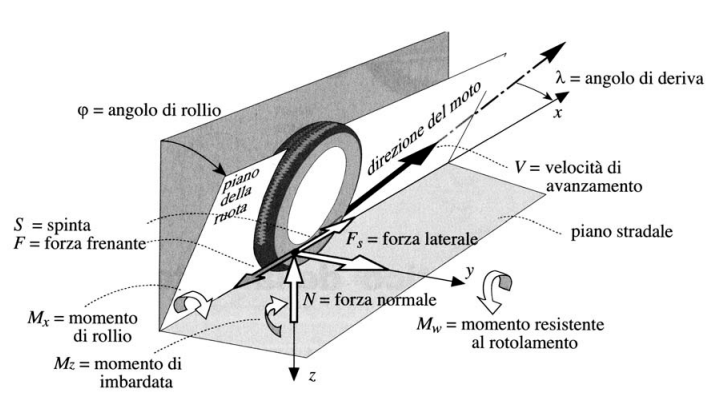
\includegraphics[scale=0.9]{Immagini/Tyres/tyre_forces.png}
    \caption{Forze e momenti generati dallo pneumatico}
    \label{fig:tyre_forces}
\end{figure}
Queste forze e momenti possono essere schematizzati come applicati in corrispondenza del centro del impronta a terra. Essi posso essere riassunti :
\begin{itemize}
    \item Una forza longitudinale, agente lungo la direzione x, assunta positiva in fase di
    accelerazione e negativa in fase di frenata. $\longrightarrow$ [$F_x$]
    \item Una forza laterale, orientata ortogonalmente a quella longitudinale ,direzione y, che garantisce la tenuta del veicolo. $\longrightarrow$ [$F_y$]
    \item Una forza normale al piano della strada, agente in direzione z. $\longrightarrow$ [$F_z$]
    \item Un momento di rollio attorno all’asse x. $\longrightarrow$ [$M_x$]
    \item Un momento di resistenza al rotolamento intorno all’asse y. $\longrightarrow$ [$M_y$]
    \item Un momento di imbardata intorno all’asse z. $\longrightarrow$ [$M_z$] 

\end{itemize}




\subsection{Magic Formula}
La Magic Formula è un modello empirico-matematico creato da Hans Bastiaan Pacejka, che che cerca di riassumere le prestazioni sperimentali dello pneumatico attraverso formule matematiche. Queste hanno una precisa struttura in cui compaiono coefficienti ricavati sperimentalmente e i parametri di funzionamento. L'obbiettivo è fornire in output varie forze e momenti che il pneumatico può generare.\\
La formulazione base è:
\begin{equation}
\label{eq:Pacjeka}
    y(x)=D*sin(C*arctant(Bx-E(Bx-arctan(Bx)))
\end{equation}
In questa formulazione la Y rappresenta la variabile in output desiderata, può essere
$F_x$, $F_y$ oppure $M_z$, $X$è la variabile in input scelta tra $\alpha$ e $k$. I Coefficenti B, C, D, E, chiamati anche coefficienti di Pacejka, esprimono:
\begin{itemize}
    \item B $\longrightarrow$ Stiffness factor \hspace{2.3cm} B $>$ 0
    \item C $\longrightarrow$ Shape factor \hspace{2.3cm} 1 $<$ C $<$ 2
    \item D $\longrightarrow$ Peak value  \hspace{2.6cm} D $= \mu*F_Z$
    \item E $\longrightarrow$ Curvature factor \hspace{2cm} E $<$ 1
\end{itemize}
I range consigliati sono presi da \cite{Guiggiani}.

\subsection{Evoluzione della Magic Formula}
La prima versione della Magic formula è stata sviluppata nel 1987 da allora sono state create una serie di nuove versioni.
Nel 1996 TNO automotive ha introdotto modello di pneumatico MF-Tyre 5.0 ed il software commerciale MF-Tool per l'estrapolazione dei parametri partendo dai dati sperimentali. Entrambi erano basati sulle equazioni presentate nell'articolo di Pacejka del 1996 \cite{Pacejka1997MagicFT}.\\ 
Nel corso degli anni sono stati apportati alcuni miglioramenti (es. aggiunta del
momento di ribaltamento, slittamento combinato migliorato, ecc.) e sono stati rilasciati i modelli: MF-Tyre 5.1 e MF-Tyre 5.2 seguentemente.\\ 
MF-Tyre è stato concepito specificatamente per autovetture e camion utilizzanti pneumatici con
angoli di inclinazione (camber) relativamente piccoli (fino a 10 gradi).\\
È stato necessario modificare le equazioni della MF, creando il modello MF-MCTyre 1.0 per poterlo utilizzare per i pneumatici delle moto che notoriamente lavorano con angoli di inclinazione molto più elevati. In una fase successiva si è migliorata la precedente versione rilasciando il MF-MCTyre 1.1.\\
Nella versione MF-Tyre 6.0 le equazioni sono state ri-adattate, in modo che un unico modello possa gestire sia i pneumatici per le auto che per le moto.
È stato aggiunto inoltre il turn slip per rappresentare, ad esempio, il momento di autoallineamento
che si verifica durante la sterzata del pneumatico a veicolo fermo.\\ 
La MF-Tyre 6.1 estende le equazioni per poter incorporare gli effetti delle variazioni nella pressione di gonfiaggio.\\
Nella MF-Tyre 6.2 il raggio di carico viene aggiornato per elevati angoli di deriva e camber. Rende inoltre disponibile l'estensione MF-Swift per motociclette. MF-Swift introduce un modello ad anello rigido, cioè si assume che la cintura del pneumatico si comporti come un corpo rigido. Questo comporta un attendibilità maggiore nella gamma di frequenze in cui la flessione della cintura del pneumatico può essere trascurata, a seconda del tipo di pneumatico siamo tra i 60 e i 100 Hz.\\ 
Il modello include gli effetti giroscopici ed utilizza un singolo punto di contatto per il calcolo dello slip; Riesce a descrivere lo slip in transitorio fino allo scorrimento completo, grazie al diminuzione della lunghezza di rilassamento all'aumentare dello slip. \\
MF-Swift è adatto per prove con raggi di curvatura che abbiano lunghezza d'onda dell'ordine di due volte la lunghezza del contatto.\\ 
\begin{figure}[!h]
    \centering
    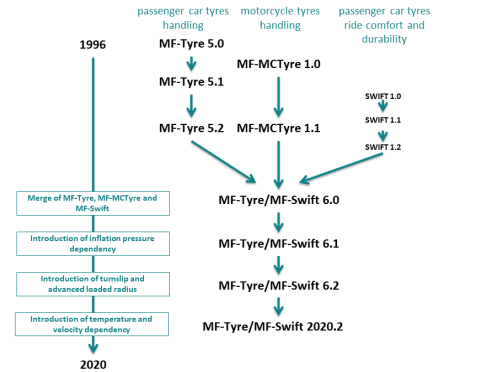
\includegraphics[scale=0.8]{Immagini/Tyres/MF-Tire History.png}
    \caption{}
    \label{fig:MF-Tire version history}
\end{figure}
\\
Per convenzione si utilizza una parola univoca che identifica la versione utilizzata è "FITTYP", questo parametro si trova nella sezione [model] del file.tir

\begin{itemize}
    {\tiny
    \setlength\itemsep{-0.5em}
    \item FITTYP = 5 \hspace{0.33cm} $\longrightarrow$ \hspace{0.2cm} MF-Tyre 5.0 , 5.1
    \item FITTYP = 6 \hspace{0.33cm} $\longrightarrow$ \hspace{0.2cm} MF-Tyre 5.2
    \item FITTYP = 21 \hspace{0.2cm} $\longrightarrow$ \hspace{0.2cm} 
    MF-Swift 1.1  (basato su MF-Tyre 5.2)
    \item FITTYP = 51 \hspace{0.2cm} $\longrightarrow$ \hspace{0.2cm} MF-MCTyre 1.0
    \item FITTYP = 52 \hspace{0.2cm} $\longrightarrow$ \hspace{0.2cm} MF-MCTyre 1.1
    \item FITTYP = 60 \hspace{0.2cm} $\longrightarrow$ \hspace{0.2cm} MF-Tyre 6.0
    \item FITTYP = 61 \hspace{0.2cm} $\longrightarrow$ \hspace{0.2cm} MF-Tyre 6.1
    \item FITTYP = 62 \hspace{0.2cm} $\longrightarrow$ \hspace{0.2cm} MF-Tyre 6.2
    \item FITTYP = 70 \hspace{0.2cm} $\longrightarrow$ \hspace{0.2cm} MF-Tyre 6.2 + Temperature and Velocity model

    }
\end{itemize}

\subsubsection{Tire property file}
Le versioni MF-Tyre precedentemente elencate sono modelli di simulazione di pneumatici definiti da una serie di parametri. Questi parametri vengono generalmente archiviati in dei file, chiamati "Tire Property File" aventi tipicamente l'estensione ".tir".\\ 
La figura \ref{fig:Structure_file_tir} mostra la classica struttura e il contenuto del file:\\
\begin{figure}[ht]
    \centering
    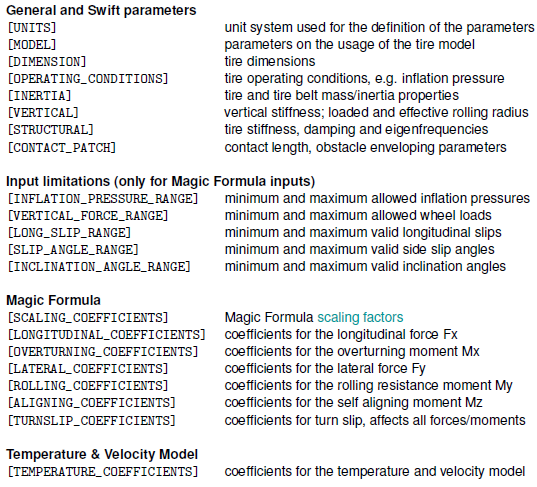
\includegraphics[scale=0.9]{Immagini/Tyres/Structure_file_tir.png}
    \caption{}
    \label{fig:Structure_file_tir}
\end{figure}
Nella prima sezione sono elencate tutte le informazioni generali , le unità di misura , tutte le caratteristiche geometriche del pneumatico
e le proprietà strutturali dello stesso.\\
Nella seconda sezione vengono elencati i limiti di pressione , forza verticale , slip e camber ai quali il modello può operare.\\
La terza sezione è la più ampia, all'interno si trovano numerosi coefficienti, di seguito elencheremo i più significativi.\\
I coefficienti di scala iniziano con la lettera L essi vengono inclusi nel file per poter ottenere un modello che simuli la realtà nel modo più affine possibile.
Come visto nell'introduzione ai pneumatici, le prove di forza e momenti vengono spesso eseguite in ambiente di laboratorio:\\ 
La superficie stradale artificiale della macchina di prova per pneumatici è usualmente molto diversa rispetto al reale manto stradale, questo, combinato all'incertezza sulla temperatura, umidità, usura, pressione di gonfiaggio, ecc., determina che il comportamento del pneumatico montato sul veicolo potrebbe discostarsi in modo significativo rispetto ai risultati ottenuti mediante la macchina di prova.\\
Verosimilmente si potrebbero avere differenze fino al 20$\%$ nel coefficiente di attrito e nella cornering stiffness \cite{Braghin2006EnvironmentalEO}.\\
I più importanti fattori di scala sono:\\
\begin{table}[h!] 
    {\scriptsize\setlength\itemsep{-0.2em}
    \centering
    \begin{tabular}{l l}
        \texttt{LMUX} \qquad \quad  & Scale factor of longitudinal peak friction coefficient\\
        \texttt{LKX} & Scale factor of longitudinal slip stiffness\\
        \texttt{LMUY} & Scale factor of lateral peak friction coefficient cornering stiffness\\
        \texttt{LKY} & Scale factor of cornering stiffness\\
        \texttt{LKYC} & Scale factor of camber stiffness\\
        \texttt{LTR} & Scale factor of pneumatic trail\\
        \texttt{LKZC} & Scale factor of camber moment stiffness\\
        \texttt{LMP} & Scale factor of parking moment at standstill\\
    \end{tabular}

    }
    \caption{}
    \label{tab:scaling factors}
\end{table}
\\
Nelle equazioni i coefficienti di scala vengono denominati attraverso il simbolo $\lambda$\\
I coefficienti della sezione 3 verranno discussi 
approfonditamente nelle successive sottosezioni.\\
La quarta sezione contiene i coefficienti per gli effetti termici e gli effetti di velocità.
Tuttavia essa si trova molto raramente per via della complessità che accompagna questi effetti.

\subsubsection{MF 5.2}
Fin dalla sua concezione, oltre 20 anni fa, la Magic Formula è stata adottata abbastanza rapidamente nell' industria come modello di pneumatico standard per simulazioni di manovrabilità dei veicoli.\\ 
Nel corso degli anni sono stati apportati vari sviluppi per
migliorare l'accuratezza ed estendere le capacità del modello.\\
Rispetto alla versione precedente (5.1), la 5.2 presenta alcune migliorie:\\
-I fattori di scala sono stati definiti in modo tale che gli effetti di conicità e plysteer possano essere facilmente disattivati.\\
-\'E stato introdotto il fattore "E", rendendo il modello più accurato in condizione di slip combinato (laterale + longitudinale).\\
-La resistenza al rotolamento è diventata funzione della velocità.\\
-Ed è stato introdotto l'effetto del Camber sul picco di forza longitudinale.\\

Il modello di pneumatico MF-Tyre 5.2 ha dimostrato una buona attendibilità ed è tuttora ampiamente utilizzato negli studi di dinamica dei veicoli. \\



Le equazioni del modello (si trovano nel MF-Tyre MF-5.2 users manual) \\
...................da completare.

\subsubsection{MF 6.1}
%Il modello MF-Tire 5.2 necessitava di alcune evoluzioni che ne ampliassero le potenzialità,
%gli obbiettivi erano:\\
Il modello MF-Tyre 6.1 rappresenta un evoluzione del 5.2, quest'ultimo infatti necessitava di alcune evoluzioni che ne ampliassero le potenzialità.\\
Nel 2010 il Dipartimento di ingegneria meccanica dell'Università di Eindhoven ha lavorato in tal senso con degli obbiettivi specifici:\\
-Migliorare la descrizione del camber, attraverso una formulazione ed un controllo espliciti sulla rigidezza al camber, estendendo inoltre le capacità del modello nel gestire angoli molto ampi (motocicli).\\
-Includere l'effetto della pressione di gonfiaggio. Questo permetteva di eliminare i numerosi file creati a diverse pressioni, in quanto consentiva di prevedere il
comportamento anche a pressioni differenti rispetto a quella con la quale si è svolto il test sperimentale, riducendo di conseguenza il numero di misurazioni richieste.\\
-Rendere coerente la descrizione della dinamica dei pneumatici tra MF-Swift e MF-Tire. Includendo l'effetto del rilassamento del pneumatico e della carcassa rigida.\\
-Migliorare la descrizione della resistenza al rotolamento e del momento di ribaltamento.\\

\begin{figure}[ht]
    \centering
    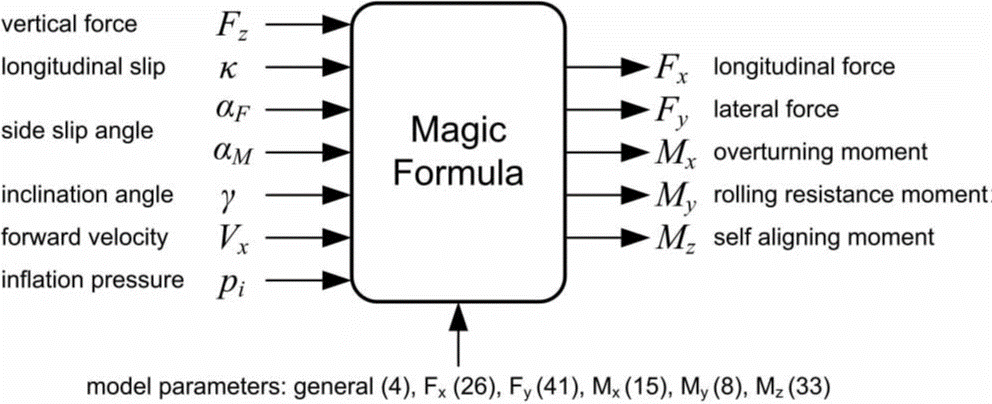
\includegraphics[scale=0.6]{Immagini/Tyres/MF.png}
    \caption{Input e output del modello MF-6.1}
    \label{fig:MF_tyres}
\end{figure}

\begin{figure}[ht]
    \centering
    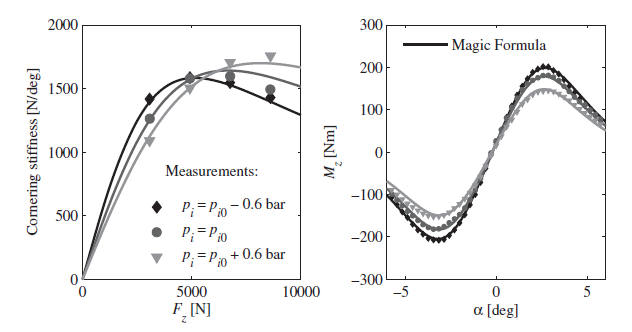
\includegraphics[scale=0.7]{Immagini/Tyres/Tyre pressure effects for a passenger car tyre.png}
    \caption{Effetto della pressione di gonfiaggio sulla cornering stiffness e sul momento di autollineamento}
    \label{fig:Pressure effects}
\end{figure}
La fig. \ref{fig:Pressure effects} mostra come al diminuire della pressione di gonfiaggio, la cornering stiffness aumenti in modo più rapido al crescere di $F_Z$ fino a valori di 5000[N] questo è dovuto al fatto .............\\
\begin{figure}[!h]
    \centering
    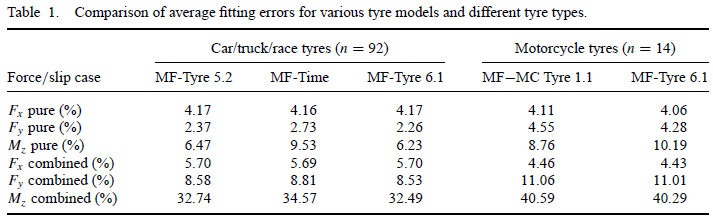
\includegraphics[scale=0.7]{Immagini/Tyres/comparison MF-Tire version.png}
    \caption{Confronto fra le versioni MF-Tire}
    \label{fig:Comparison MF-Tire version}
\end{figure}
La fig. \ref{fig:Comparison MF-Tire version} mostra un confronto tra la media degli errori di fitting.\\  
Le fig. \ref{fig:Pressure effects} e \ref{fig:Comparison MF-Tire version} sono prese da \cite{Besselink2010AnIM}.\\

\section{Dinamica Laterale}
In questo capitolo verranno descritte le basi della dinamica del veicolo per quanto concerne la dinamica laterale.\\
Il comportamento dinamico di un veicolo può essere suddiviso in: longitudinale (trazione
e frenata), laterale (handling) e verticale (comfort).
In questa trattazione ci occuperemo del comportamento laterale cioè l'insieme delle risposte dinamiche in direzione perpendicolare alla direzione del moto, che il veicolo restituisce in risposta agli input forniti dal guidatore (sterzo e velocità).\\
Le fonti di questo argomento sono \cite{Guiggiani} e \cite{limebeer2018dynamics}, mentre ulteriori approfondimenti si trovano in  \cite{pacejka2005tire}.\\



In questa prima analisi il veicolo viene considerato un unico corpo rigido in
moto su un piano, dunque avente tre gradi di libertà: due traslatori e uno
rotatorio con asse perpendicolare al piano considerato.\\ 
Per l'analisi (quasi)-stazionaria verranno utilizzati semplici modelli di veicoli. 


\subsection{Single track model}
Il modello a singola traccia anche chiamato impropriamente (in gergo) modello a "bicicletta" è il modello più semplice utilizzato per analizzare le dinamiche laterali dei veicoli.\\
\'E molto utile per comprendere i fenomeni di handling in quanto presenta il vantaggio dell'essere semplice ed intuitivo permettendo una rapida valutazione dell'influenza dei parametri caratteristici.\\
\begin{figure}[!h]
    \centering
    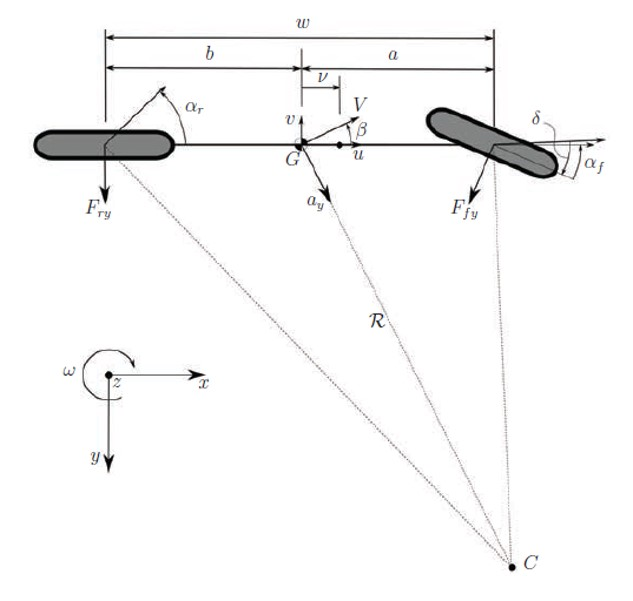
\includegraphics[scale=0.7]{Immagini/Lateral dynamics/Single_track_model.jpg}
    \caption{cinematica del single track model}
    \label{fig:Single track model}
\end{figure}
Ammettendo la simmetria rispetto all’asse longitudinale,
il veicolo può esser rappresentato da una sola linea con alle estremità i due
pneumatici (assale posteriore e anteriore sono condensati in due singole "
ruote equivalenti").\\
la fig. \ref{fig:Single track model} è la rappresentazione, appunto, della vista dall'alto di un veicolo privo di larghezza ,si tratta di un corpo rigido di massa $m$ concentrata nel centro di massa G, le cui distanze $a$ e $b$ sono i due semipassi,
rispettivamente anteriore e posteriore. Con $L$ o $W$ si indica il passo, cioè la distanza tra asse anteriore e posteriore.\\
%\singlespace 
Inoltre è possibile definire:
\begin{itemize}
    \begin{spacing}{1}
    \setlength\itemsep{-0.1em}
    \item \textbf{Velocità longitudinale} ($u$) : velocità di avanzamento in direzione longitudinale al veicolo.
    \item \textbf{Velocità laterale} ($v$) : velocità di scorrimento laterale del veicolo
    \item \textbf{Velocità d'imbardata} ($r$) : velocità angolare rispetto all'asse verticale z del sistema di riferimento assoluto
    \item \textbf{Angolo di assetto} ($\beta$) : angolo formato tra la direzione del vettore velocità assoluta e la direzione longitudinale del veicolo.
    \item \textbf{Angoli di deriva} ($\alpha_f$) e ($\alpha_r$) : angoli formati tra il piano medio della ruota (anteriore o posteriore) ed il vettore velocità del centro del impronta di contatto.
    \item \textbf{Angolo di sterzo} ($\delta$) : angolo formato tra l'asse di simmetria del veicolo ed il piano della ruota.
    \end{spacing}
\end{itemize}
Questo modello ignora gli effetti delle sospensioni, del telaio e del trasferimento del carico laterale.\\
\subsubsection{Equazioni di equilibrio}
La velocità assoluta del centro di massa può essere espressa attraverso i versori del sistema di riferimento del veicolo:\\
\begin{equation}
\textbf{V} = u\textbf{i}+v\textbf{j}
\end{equation}
L'accelerazione laterale è data:\\
\begin{equation}
\begin{split}
\frac{d\textbf{V}}{dt} & = \textbf{$\dot V$}+r\textbf{k}\times\textbf{V}\\
 & = \hat{a_x}\textbf{i}+\hat{a_y}\textbf{j}
\end{split}
\end{equation}
$\hat{a_x}$ è l'accelerazione longitudinale mentre $\hat{a_y}$ è accelerazione laterale normale al piano di simmetria del veicolo.\\
\begin{align}
\hat{a_x} & = \dot u - rv\\
\hat{a_y} & = \dot v + ru
\end{align}
Imponendo l'equilibrio delle forze in direzione longitudinale e laterale e dei momenti si ottengono le seguenti equazioni del moto:
\begin{align}
m(\dot u- rv) & = -F_{yf} \sin \delta+F_{xf} \cos \delta+F_{xr}\\
m(\dot v+ ru) & = +F_{yf} \cos \delta+F_{xf} \sin \delta+F_{yr}\\
J\dot r & = a*(F_{yf} \cos \delta+F_{xf} \sin \delta)-b*F_{yr}\\[3mm]
m\dot u & =  mrv-F_{yf} \sin \delta+F_{xf} \cos \delta+F_{xr} \label{eq:eom longitudinal}\\
m\dot v & = -mru+F_{yf} \cos \delta+F_{xf} \sin \delta+F_{yr} \label{eq:eom lateral}\\
J\dot r & = a*(F_{yf} \cos \delta+F_{xf} \sin\delta)-b*F_{yr} \label{eq:eom yaw}
\end{align}
Nelle quali $m$ e $J$ sono rispettivamente la massa ed il momento d'inerzia all'imbardata, mentre $u$, $v$, e $r$ sono le variabili di stato del modello.
Per veicoli a trazione posteriore (RWD) e ipotesi di resistenza al rotolamento nulla, la $F_{fx}$ è trascurabile.\\
Inoltre approssimando il $sin(\delta)=0$ e $cos(\delta)=1$, l'eq.\ref{eq:eom longitudinal} 
risulta disaccoppiata e dunque ininfluente nello studio delle dinamiche laterali\\
Rimangono di conseguenza solo le \ref{eq:eom lateral} e \ref{eq:eom yaw} che diventano:
\begin{align}
m\dot v & = -mru+F_{yf}+F_{yr}\label{eq:eom lateral 2}\\
J\dot r & = a*F_{yf}-b*F_{yr}\label{eq:eom yaw 2}
\end{align}

\subsubsection{Equazioni cinematiche}
I tre angoli di deriva possono essere calcolati utilizzando le seguenti relazioni cinematiche:
\begin{align}
\beta & = \arctan(\frac{v}{u})\\
\alpha_f & = \delta - \arctan(\frac{ra+v}{u})\\
\alpha_r & = \arctan(\frac{rb-v}{u})
\end{align}
Nell'ipotesi di piccoli angoli queste possono essere approssimate
\begin{align}
\beta & = \frac{v}{u}\\
\alpha_f & = \delta - \frac{ra+v}{u} \label{eq:alfa front} \\
\alpha_r & = \frac{rb-v}{u} \label{eq: alfa rear}
\end{align}
Definiamo con $R$ il raggio di curvatura : $R=\frac{u}{r}$.\\
Mentre la Curvatura è l'inverso del raggio di curvatura dunque $\rho = \frac{1}{R} = \frac{r}{u}$.\\
Attraverso l'equilibrio delle forze in direzione Z si ricavano i carichi verticali (statici) sui singoli assi:
\begin{align}
F_{zf} & = mg \frac{b}{a+b}\\
F_{zr} & = mg \frac{a}{a+b}
\end{align}

\subsubsection{Modello monotraccia lineare}
Si può riepilogare quanto visto finora attraverso il modello monotraccia lineare, Abbiamo visto nella sezione pneumatici come essi possano essere semplificati in modo puramente teorico con l' equazione costitutiva lineare dove la forza laterale generata è funzione dell'angolo di deriva moltiplicato per la rigidezza (cornering stiffness).
\begin{equation}
    \label{eq:Fy=C*alfa}
    F_{y,i} = C_i*\alpha_i
\end{equation}
Introducendo in quest'ultima equazione le equazioni cinematiche degli angoli di slip \ref{eq:alfa front} e \ref{eq: alfa rear} otteniamo:\\
\begin{align}
F_{yf} & = C_f*\alpha_f = C_f*(\delta - \frac{ra+v}{u}) \\
F_{yr} & = C_r*\alpha_r = C_r*(\frac{rb-v}{u}) 
\end{align}
Sostituendo queste due equazioni all'interno delle equazioni di equilibrio \ref{eq:eom lateral 2} e \ref{eq:eom yaw 2} otteniamo le seguenti equazioni del moto:
\begin{align}
m\dot v & = -mru + C_f\delta  + ( C_f - C_r)\frac{v}{u} + (- C_fa + C_rb)\frac{r}{u}\label{eq:eom lateral linear}\\
J\dot r & = aC_f\delta + (C_f a^2 + C_r b^2)\frac{r}{u} + ( C_fa - C_rb)\frac{v}{u}\label{eq:eom yaw linear}
\end{align}
\begin{align}
\dot v & = \frac{ C_f - C_r}{mu}v + \frac{- C_fa + C_rb}{mu}r - \frac{u}{m}r + \frac{C_f}{m}\delta\label{eq:eom lateral linear}\\
\dot r & = \frac{ C_fa - C_rb}{Ju}v + \frac{C_f a^2 + C_r b^2
}{Ju}r + \frac{aC_f}{J}\delta \label{eq:eom yaw linear}
\end{align}
In condizioni quasi-statiche le accelerazioni sono nulle dunque:
\begin{align}
0 & = \frac{ C_f - C_r}{mu}v + \frac{- C_fa + C_rb}{mu}r - ur + \frac{C_f}{m}\delta\\
0 & = \frac{ C_fa - C_rb}{Ju}v + \frac{C_f a^2 + C_r b^2}{Ju}r + \frac{aC_f}{J}\delta 
\end{align}
Questo è un sistema di due equazioni e due incognite $v$ e $r$ nel quale $u$ e $\delta$ sono gli input.\\
Introducendo la notazione matriciale il sistema \ref{eq:eom lateral linear} \ref{eq:eom yaw linear} può essere rappresentato attraverso le matrici A e B.\\
\begin{equation}
\begin{Bmatrix}
\dot v\\
\dot r
\end{Bmatrix}
=
\underbrace{\begin{bmatrix}
\frac{ C_f - C_r}{mu} & \frac{- C_fa + C_rb}{mu} - u\\
\frac{ C_fa - C_rb}{Ju}  & \frac{C_f a^2 + C_r b^2}{Ju} 
\end{bmatrix}}_{A}
\begin{Bmatrix}
v\\
r
\end{Bmatrix}
\underbrace{\begin{bmatrix}
\frac{C_f}{m}\\
\frac{aC_f}{J} 
\end{bmatrix}}_{B}
\begin{Bmatrix}
\delta
\end{Bmatrix}
\end{equation}
In condizioni di regime ricaviamo la velocità laterale e la velocità angolare d'imbardata :
\begin{equation}
\begin{Bmatrix}
v\\
r
\end{Bmatrix}
=
\begin{bmatrix}
A 
\end{bmatrix}^{-1}
\begin{bmatrix}
B 
\end{bmatrix}
\begin{Bmatrix}
\delta
\end{Bmatrix}
\end{equation}

\subsubsection{Stabilità del modello}
Per lo studio della stabiità di marcia del modello è necessario analizzarlo in seguito ad una perturbazione rispetto alla condizione di equilibrio.
La risposta sarà una combinazione di modi di vibrare.
Un sistema è stabile quando i tutti suoi modi di vibrare hanno parte reale negativa, basta un singolo modo di vibrare con parte reale positiva e il sistema sarà instabile.\\
Le radici del polinomio caratteristico sono appunto i modi di vibrare.\\
Imponendo il $det[SI-A]=0$ troviamo gli autovalori:
\begin{gather}det
    \begin{bmatrix}
    S-\frac{ C_f - C_r}{mu} & \frac{ C_fa - C_rb}{mu} - u\\
    \frac{ -C_fa + C_rb}{Ju}  & S-\frac{C_f a^2 + C_r b^2}{Ju} 
    \end{bmatrix} = 0 \\
    \begin{bmatrix}
        S^2 - S\frac{C_f a^2 + C_r b^2}{Ju} - S\frac{C_f-C_r}{mu} + \frac{C_f-C_r}{mu}\frac{C_f a^2 + C_r b^2}{Ju}
    \end{bmatrix}
    -
    \begin{bmatrix}
        \frac{(C_fa-C_rb)^2}{mJu} + \frac{C_fa-C_rb}{J}
    \end{bmatrix} = 0\\
    \underbrace{\begin{bmatrix}
    1
    \end{bmatrix}}_{a_2}S^2 +
    \underbrace{\begin{bmatrix}
    \frac{C_f a^2 - C_r b^2}{Ju} + \frac{C_f+C_r}{mu}
    \end{bmatrix}}_{a_1} S +
    \underbrace{\begin{bmatrix}
    \frac{C_f-C_r}{mu}\frac{C_f a^2 + C_r b^2}{Ju} - \frac{(C_fa-C_rb)^2}{mJu} - \frac{C_fa-C_rb}{J}
    \end{bmatrix}}_{a_0} = 0
\end{gather}
Secondo il criterio di Hurwitz un sistema è stabile quando tutti i coefficienti del polinomio caratteristico hanno lo stesso segno.
Essendo $a_2$ e $a_1$ positivi, affinche il sistema sia stabile dovrà essere positivo anche $a_0$.
imponendo questa condizione otteniamo che affinchè il sistema sia stabile
\begin{equation}
    \begin{split}
        u^2 & < -\frac{C_f C_r (a+b)}{C_rb-C_fa} \frac{(a+b)}{m} \\
            & < -\frac{C_f C_r (a+b)}{mg(C_rb-C_fa)} (a+b)*g \\
          u & < \sqrt{-\frac{g(a+b)}{\zeta}}
    \end{split}
\end{equation}
Definiamo dunque la velocità critica valida solo per veicoli sovrasterzanti ($\zeta < 0$)
\begin{equation}
    u_{cr} = \sqrt{-\frac{g(a+b)}{\zeta}}
\end{equation}
Introduciamo ora il gradiente di sottosterzo per il modello lineare:
\begin{equation}
    \zeta = \frac{C_rb-C_fa}{C_f C_r (a+b)}*mg
\end{equation}
\begin{enumerate}
    \item Se $C_rb-C_fa < 0$ ($\zeta < 0$) il veicolo si definisce \textbf{sovrasterzante}
    \item Se $C_rb-C_fa = 0$ ($\zeta < 0$) il veicolo si definisce \textbf{neutro}
    \item Se $C_rb-C_fa > 0$ ($\zeta > 0$) il veicolo si definisce \textbf{sottosterzante}
\end{enumerate}
Ovvero se la capacità direttiva del retrotreno ($C_rb$) è maggiore della capacità direttiva dell'avantreno ($C_fa$) il
veicolo è detto sottosterzante in quanto il raggio di curvatura che percorre sarà maggiore del raggio di curvatura che 
dovrebbe percorrere dato dalla combinazione di velocità e angolo di sterzo. 
Questo argomento verrà trattato approfonditamente nel cap.\ref{cha:cap2}.

\subsection{Double track model}
Il modello a doppia traccia è l'evoluzione del modello a singola traccia, in questo caso il veicolo viene rappresentato attraverso la sua vista dall'alto con quattro ruote.\\
Questo modello permette di considerare gli effetti sul comportamento direzionale del trasferimento di carico laterale, della sterzata di Ackermann e toe, del camber e dell'aerodinamica.\\
Come nel caso precedente la dinamica longitudinale verrà trascurata in quanto non è argomento di tesi.\\

\begin{figure}[ht]
    \centering
    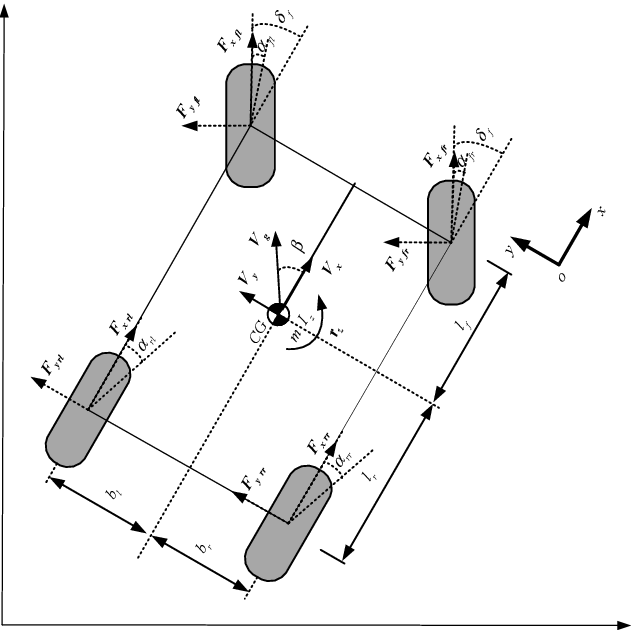
\includegraphics[scale=0.4]{Immagini/Lateral dynamics/Double-track-model-of-vehicle-lateral-dynamics.png}
    \caption{Double track model}
    \label{fig:Double track model}
\end{figure}
Come nel caso precedente possiamo scrivere le equazioni del moto: 
\begin{align}
\\
m(\dot u- rv) & = F_{xrl} + F_{xrr} + F_{xfl} \cos \delta_l + F_{xfr} \cos \delta_r -F_{yfl} \sin \delta_l -F_{yfr} \sin \delta_r\\
m(\dot v+ ru) & = F_{yrl} + F_{yrr} + F_{yfl} \cos \delta_l + F_{yfr} \cos \delta_r +F_{xfl} \sin \delta_l +F_{xfr} \sin \delta_r\\
J\dot r & = a*(F_{yfl} \cos \delta_l + F_{yfr} \cos \delta_r +F_{xfl} \sin \delta_l +F_{xfr} \sin \delta_r)-b*(F_{yrl} + F_{yrr})
\end{align}
Ipotizzando $F_{xrl}=F_{xrr}$ le coppie differenziali posteriori sono nulle.\\
Gli angoli di deriva laterali risultano:
\begin{align}
\alpha_{fl} & = - (\frac{ra+v}{u+r\frac{Wt_{f}}{2}}) + \delta_f\\
\alpha_{fr} & = - (\frac{ra+v}{u-r\frac{Wt_{f}}{2}}) + \delta_r\\
\alpha_{rl} & = - (\frac{-rb+v}{u+r\frac{Wt_{r}}{2}})\\
\alpha_{rr} & = - (\frac{-rb+v}{u-r\frac{Wt_{r}}{2}})
\end{align}


\subsubsection{Trasferimento di carico laterale}
Il rollio è la rotazione veicolo attorno all'asse di rollio , è un asse parallelo all'asse longitudinale dello stato individuato dalla retta che unisce i centri di rollio dell'asse anteriore e dell'asse posteriore.\\
Il rollio avviene nei veicoli dotati di sospensioni durante una curva, a seguito della forza centrifuga generata, questa agendo sulla massa sospesa tende ad inclinarla nel direzione opposta rispetto alla direzione della curva.\\
La forza peso del veicolo tende ad aumentare nelle ruote esterne e diminuire nelle ruote interne.\\
\begin{align}
F_{zfl} & = mg \frac{b}{a+b} + m a_y \frac{h}{Wt_f} D + \frac{Faero_f}{2}\\
F_{zfr} & = mg \frac{b}{a+b} - m a_y \frac{h}{Wt_f} D + \frac{Faero_f}{2}\\
F_{zrl} & = mg \frac{a}{a+b} + m a_y \frac{h}{Wt_f} (1-D) + \frac{Faero_r}{2}\\
F_{zrr} & = mg \frac{a}{a+b} - m a_y \frac{h}{Wt_f} (1-D) + \frac{Faero_r}{2}
\end{align}
Definiamo con D il mechanical balance, un parametro che indica come si distribuirà il trasferimento di carico laterale tra assale anteriore e assale posteriore.
\begin{equation}
    D = \frac{K_{\phi f}}{K_\phi}\frac{h-d}{h} + \frac{b}{L} \frac{d_f}{h} \label{eq:Mechanical balance}
\end{equation}
Come si può vedere dall'eq.\ref{eq:Mechanical balance} questo parametro è funzione di :\\
$\bullet K_{\phi f}$ è la rigidezza torsionale dell'assale anteriore comprende le varie rigidezze delle sospensioni e delle eventuali barre di torsione presenti\\
$\bullet K_{\phi}$ è la rigidezza torsionale complessiva del veicolo, è la somma di $K_{\phi f}$ e $K_{\phi r}$.\\
$\bullet h$ è l'altezza del centro di massa rispetto al piano di appoggio.\\
$\bullet d_f$ è l'altezza del centro di rollio dell'asse anteriore.\\
$\bullet h$ è l'altezza del punto formato dall'intersezione tra l'asse di rollio e la retta verticale a distanza $a$ dall'asse anteriore.
(inserire figura con le quote).

\subsubsection{Ackermann steering}

\begin{figure}[ht]
    \centering
    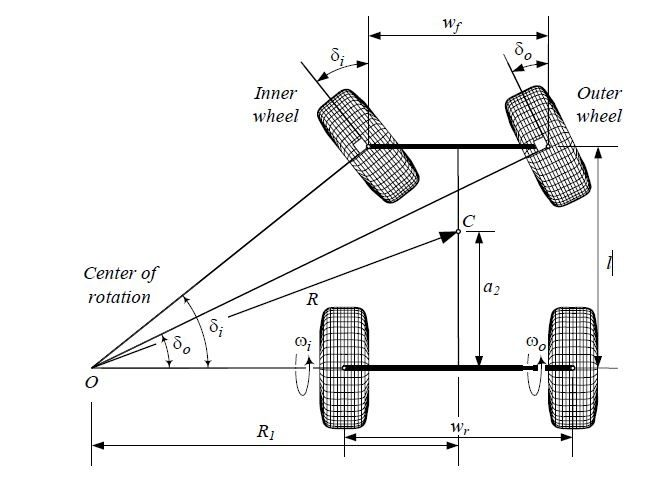
\includegraphics[scale=0.4]{Immagini/Lateral dynamics/Angolo-di-Ackermann.jpg}
    \caption{Sterzata di Ackermann}
    \label{fig:Ackermann}
\end{figure}

\subsubsection{Camber}
L'angolo di camber o "di campanatura" è l'angolo formato tra l'asse verticale passante per il centro dell'impronta di contatto dello pneumatico e l'asse radiale della ruota.
il camber statico è l'angolo misurato a veicolo fermo mentre il camber dinamico è funzione della cinematica delle sospensioni e dunque del trasferimento di carico.

\begin{figure}[ht]
    \centering
    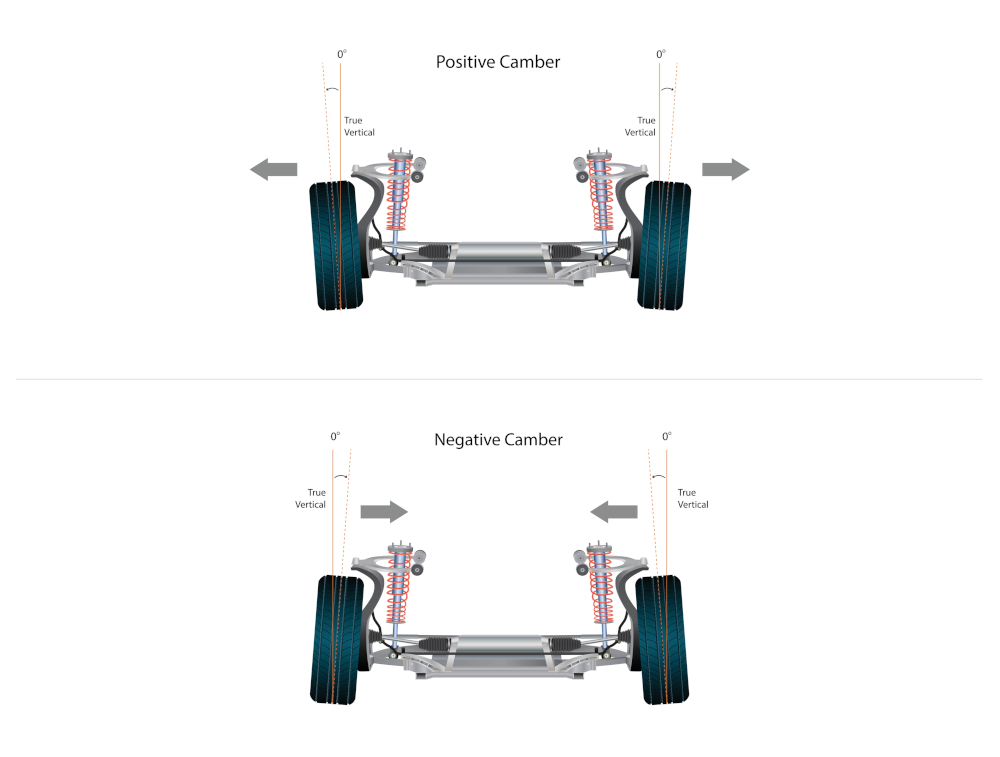
\includegraphics[scale=0.4]{Immagini/Lateral dynamics/Camber.jpg}
    \caption{Angoli di Camber}
    \label{fig:Camber}
\end{figure}


\subsubsection{Convergenza delle ruote}

\begin{figure}[ht]
    \centering
    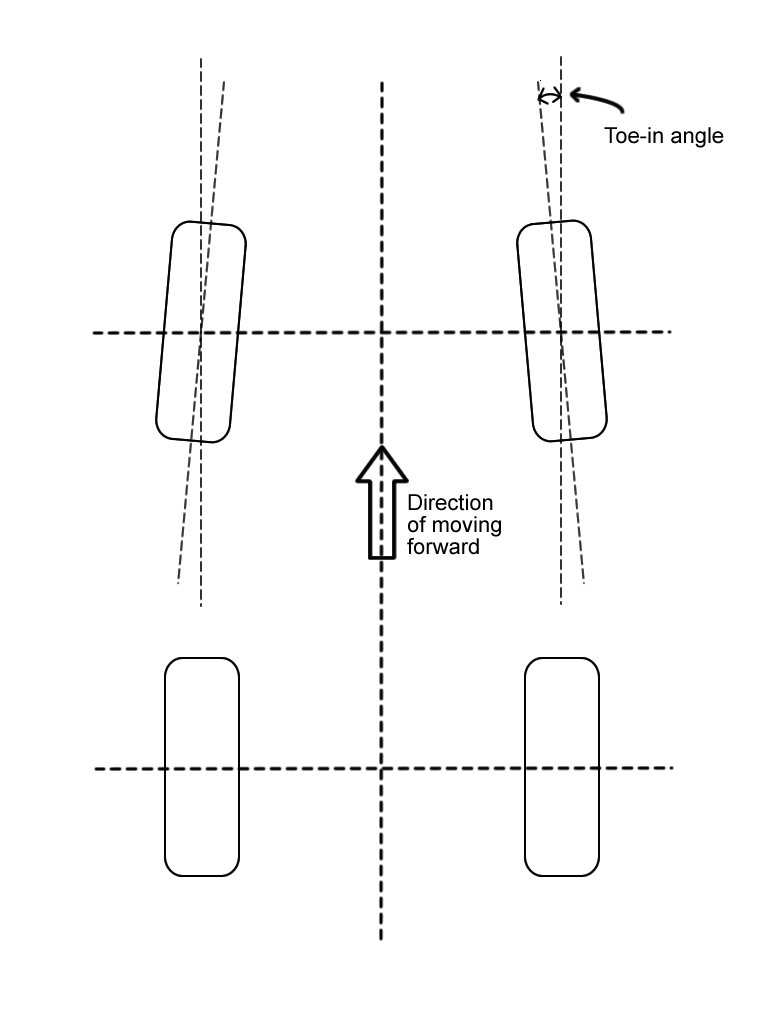
\includegraphics[scale=2]{Immagini/Lateral dynamics/Toe-in.png}
    \caption{Convergenza delle ruote anteriori}
    \label{fig:Toe-in}
\end{figure}

\subsubsection{Aerodinamica}